\def\DoNotLoadEpstopdf{}
\documentclass[tikz,border=4pt]{standalone}
% Shared style for the technical appendix figures (2026-10-26).
% Builds on the proposal's figstyle.tex (same fonts, colors, and box styles) and adds
% one encoding for development status, used the same way in every appendix figure.
%   built and tested   solid border (the proposal's normal box styles)
%   built, no test     solid border, and the box text says "no test"
%   specified          dashed border            -> add the key  spec
%   planned            dotted grey border        -> use the style planned
%   no code (by hand)  dotted arrow              -> add the key  byhand
%   outside the artifact  solid grey border      -> use the style outside
% Shared style for proposal figures (2026-10-22 visuals pass).
% Sized to print at 6.5 in (16.5 cm) wide; body text 9 pt sans, nothing below 8 pt.
\usepackage[T1]{fontenc}
\usepackage[scaled=0.95]{helvet}
\renewcommand{\familydefault}{\sfdefault}
\usepackage{xcolor}
\usetikzlibrary{arrows.meta,positioning,calc,patterns.meta}
\definecolor{cink}{HTML}{16191F}
\definecolor{cmuted}{HTML}{4B5563}
\definecolor{cslate}{HTML}{2F4858}
\definecolor{cslatefill}{HTML}{E9EFF3}
\definecolor{cbrass}{HTML}{7A5C12}
\definecolor{cbrassfill}{HTML}{F5EFDE}
\definecolor{cred}{HTML}{8C2F39}
\definecolor{credfill}{HTML}{F8E9EA}
\definecolor{cgreen}{HTML}{235C53}
\definecolor{cgreenfill}{HTML}{E3F0EC}
\definecolor{caudit}{HTML}{5B3A8E}
\definecolor{cauditfill}{HTML}{EFE9F6}
\definecolor{cghost}{HTML}{6B7280}
\definecolor{cghostfill}{HTML}{F3F4F6}
\tikzset{
  >={Triangle[length=5pt,width=4.5pt]},
  box/.style={draw, rounded corners=1.5pt, line width=0.8pt, align=center, inner sep=4pt, font=\fontsize{9}{11}\selectfont},
  sub/.style={font=\fontsize{8}{9.6}\selectfont, text=cmuted},
  ai/.style={box, draw=cbrass, fill=cbrassfill, text=cbrass},
  ver/.style={box, draw=cred, fill=credfill, text=cred},
  pipe/.style={box, draw=cslate, fill=cslatefill, text=cslate},
  prod/.style={box, draw=cslate, fill=cslate, text=white},
  person/.style={box, draw=cink, fill=white, text=cink},
  ghost/.style={box, draw=cghost, fill=cghostfill, text=cghost, dash pattern=on 3pt off 2pt},
  flow/.style={->, line width=0.8pt},
}

\renewcommand{\ttdefault}{lmtt}% vector typewriter font (same design as the default, not a bitmap)
\tikzset{
  spec/.style={dash pattern=on 3pt off 2pt},
  planned/.style={box, draw=cghost, fill=cghostfill, text=cghost, dash pattern=on 0.9pt off 1.6pt},
  outside/.style={box, draw=cghost, fill=white, text=cghost},
  byhand/.style={dash pattern=on 0.9pt off 1.6pt},
  prog/.style={font=\fontsize{8}{9.6}\selectfont\ttfamily},
  legendbox/.style={draw, rounded corners=1pt, line width=0.8pt, minimum width=0.55cm, minimum height=0.32cm, inner sep=0pt},
  legendtext/.style={font=\fontsize{8}{9.6}\selectfont, text=cink, anchor=west, inner sep=1pt},
}
% \statuslegend{x}{y} draws the four-item status legend with its left edge at (x,y).
\newcommand{\statuslegend}[2]{%
  \begin{scope}[shift={(#1,#2)}]
    \node[legendbox, draw=cink, fill=white] (lg1) at (0.275,0) {};
    \node[legendtext] at (0.65,0) {Built and tested};
    \node[legendbox, draw=cink, fill=white, spec] (lg2) at (3.35,0) {};
    \node[legendtext] at (3.725,0) {Specified};
    \node[legendbox, draw=cghost, fill=cghostfill, dash pattern=on 0.9pt off 1.6pt] (lg3) at (5.75,0) {};
    \node[legendtext] at (6.125,0) {Planned};
    \node[legendbox, draw=cghost, fill=white] (lg4) at (7.85,0) {};
    \node[legendtext] at (8.225,0) {Outside the research artifact};
  \end{scope}}

\usetikzlibrary{backgrounds}
\begin{document}
\hyphenpenalty=10000
\newcommand{\pg}[1]{{\ttfamily #1}}
\newcommand{\sm}[1]{{\color{cmuted}#1}}
\newcommand{\hd}[1]{{\fontsize{9}{9.6}\selectfont\bfseries #1}}
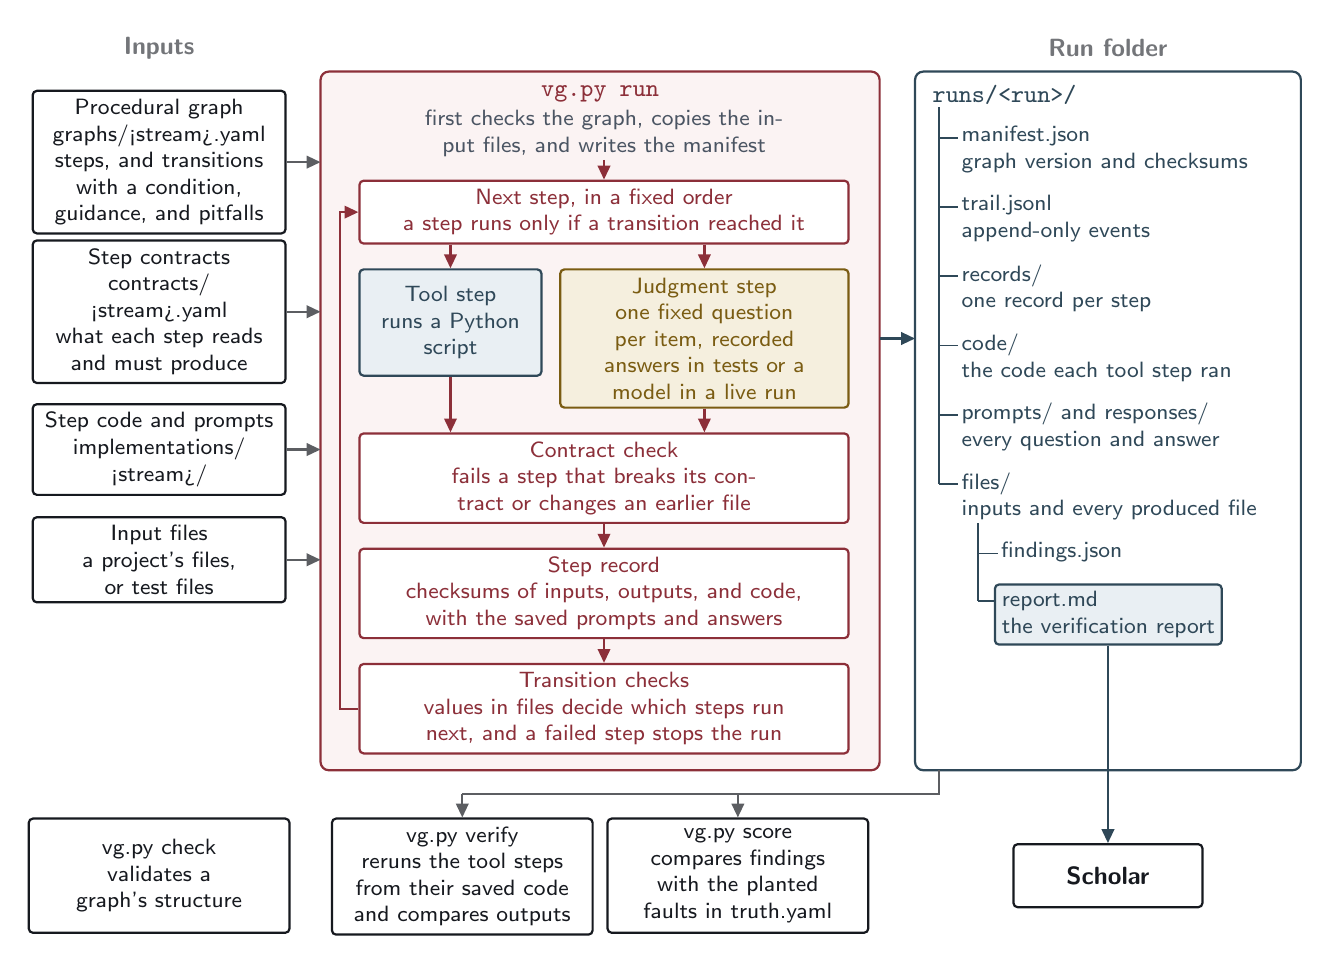
\begin{tikzpicture}[node distance=0.3cm]
\tikzset{
  small/.style={font=\fontsize{8}{9.6}\selectfont},
  inp/.style={person, small, text width=3.0cm, minimum width=3.2cm, inner sep=3pt},
  st/.style={box, small, draw=cred, fill=white, text=cred, text width=6.0cm, minimum width=6.2cm, inner sep=3pt},
  cmd/.style={person, small, text width=3.1cm, minimum width=3.3cm, inner sep=3pt, minimum height=1.45cm},
  rflow/.style={->, line width=0.8pt, cred},
  head/.style={font=\fontsize{9}{11}\selectfont\bfseries, text=cink!60},
  ent/.style={small, anchor=west, align=left, inner sep=1pt, text=cslate},
}
% ---------------------------------------------------------------- headings
\node[head] at (1.6,10.95) {Inputs};
\node[head] at (13.65,10.95) {Run folder};

% ---------------------------------------------------------------- runtime frame

\node[font=\fontsize{9}{11}\selectfont\ttfamily, text=cred, anchor=north] (title) at (7.2,10.6) {vg.py run};
\node[small, text width=6.3cm, align=center, anchor=north, inner sep=1pt, text=cmuted] (init) at (7.25,10.2) {first checks the graph, copies the input files, and writes the manifest};

\node[st, below=0.25cm of init] (next) {\hd{Next step, in a fixed order}\\\sm{a step runs only if a transition reached it}};
\node[pipe, small, text width=2.1cm, minimum width=2.3cm, minimum height=1.35cm, inner sep=3pt, below=0.3cm of next.south west, anchor=north west] (tool) {\hd{Tool step}\\\sm{runs a Python script}};
\node[ai, small, text width=3.45cm, minimum width=3.65cm, minimum height=1.35cm, inner sep=3pt, below=0.3cm of next.south east, anchor=north east] (judge) {\hd{Judgment step}\\\sm{one fixed question per item, recorded answers in tests or a model in a live run}};
\coordinate (cj) at (next.south |- judge.south);
\node[st, below=0.3cm of cj, anchor=north] (contract) {\hd{Contract check}\\\sm{fails a step that breaks its contract or changes an earlier file}};
\node[st, below=0.3cm of contract] (record) {\hd{Step record}\\\sm{checksums of inputs, outputs, and code, with the saved prompts and answers}};
\node[st, below=0.3cm of record] (trans) {\hd{Transition checks}\\\sm{values in files decide which steps run next, and a failed step stops the run}};

\path (trans.south) ++(0,-0.2) coordinate (fb);
\begin{pgfonlayer}{background}
\draw[cred, fill=credfill!55, line width=0.8pt, rounded corners=3pt] (3.65,0 |- fb) rectangle (10.75,10.65);
\draw[cslate, line width=0.8pt, rounded corners=3pt] (11.2,0 |- fb) rectangle (16.1,10.65);
\end{pgfonlayer}
\draw[rflow] (init) -- (next);
\draw[rflow] (next.south -| tool.north) -- (tool.north);
\draw[rflow] (next.south -| judge.north) -- (judge.north);
\draw[rflow] (tool.south) -- (tool.south |- contract.north);
\draw[rflow] (judge.south) -- (judge.south |- contract.north);
\draw[rflow] (contract) -- (record);
\draw[rflow] (record) -- (trans);
\draw[rflow] (trans.west) -- (3.9,0 |- trans.west) -- (3.9,0 |- next.west) -- (next.west);

% ---------------------------------------------------------------- inputs
\node[inp] (graph) at (1.6,9.5) {\hd{Procedural graph}\\\pg{graphs/<stream>.yaml}\\\sm{steps, and transitions with a condition, guidance, and pitfalls}};
\node[inp] (contr) at (1.6,7.6) {\hd{Step contracts}\\\pg{contracts/}\\\pg{<stream>.yaml}\\\sm{what each step reads and must produce}};
\node[inp] (impl) at (1.6,5.85) {\hd{Step code and prompts}\\\pg{implementations/}\\\pg{<stream>/}};
\node[inp] (infiles) at (1.6,4.45) {\hd{Input files}\\\sm{a project's files, or test files}};
\foreach \n in {graph,contr,impl,infiles} {\draw[flow, cink!70] (\n.east) -- (3.65,0 |- \n.east);}

% ---------------------------------------------------------------- run folder

\node[anchor=north west, font=\fontsize{9}{11}\selectfont\ttfamily, text=cslate] at (11.3,10.6) {runs/<run>/};
\tikzset{ent/.append style={anchor=north west}}
\def\ex{11.75}
\node[ent] (man) at (\ex,10.0) {\pg{manifest.json}\\\sm{graph version and checksums}};
\node[ent] (trl) at (\ex,9.12) {\pg{trail.jsonl}\\\sm{append-only events}};
\node[ent] (rec) at (\ex,8.24) {\pg{records/}\\\sm{one record per step}};
\node[ent] (cod) at (\ex,7.36) {\pg{code/}\\\sm{the code each tool step ran}};
\node[ent] (pr) at (\ex,6.48) {\pg{prompts/} \sm{and} \pg{responses/}\\\sm{every question and answer}};
\node[ent] (fi) at (\ex,5.6) {\pg{files/}\\\sm{inputs and every produced file}};
\node[ent] (find) at (12.25,4.72) {\pg{findings.json}};
\node[box, small, draw=cslate, fill=cslatefill, text=cslate, anchor=north west, align=left, inner sep=2.5pt] (rep) at (12.2,4.15) {\pg{report.md}\\\sm{the verification report}};
\foreach \n in {man,trl,rec,cod,pr,fi,find} {\coordinate (t\n) at ($(\n.north west)+(0,-0.19)$);}
\coordinate (trep) at ($(rep.north west)+(0,-0.22)$);
\draw[cslate, line width=0.6pt] (11.5,10.2) -- (11.5,0 |- tfi);
\foreach \n in {man,trl,rec,cod,pr,fi} {\draw[cslate, line width=0.6pt] (11.5,0 |- t\n) -- (t\n);}
\draw[cslate, line width=0.6pt] (12.0,0 |- fi.south) -- (12.0,0 |- trep);
\draw[cslate, line width=0.6pt] (12.0,0 |- tfind) -- (tfind);
\draw[cslate, line width=0.6pt] (12.0,0 |- trep) -- (trep);

% runtime writes the run folder
\draw[flow, cslate] (10.75,0 |- judge) -- (11.2,0 |- judge);

% ---------------------------------------------------------------- after the run
\path (fb) ++(0,-0.6) coordinate (bt);
\node[cmd, anchor=north] (chk) at (1.6,0 |- bt) {\pg{vg.py check}\\\sm{validates a graph's structure}};
\node[cmd, anchor=north] (ver) at (5.45,0 |- bt) {\pg{vg.py verify}\\\sm{reruns the tool steps from their saved code and compares outputs}};
\node[cmd, anchor=north] (sco) at (8.95,0 |- bt) {\pg{vg.py score}\\\sm{compares findings with the planted faults in \pg{truth.yaml}}};
\node[person, minimum width=2.4cm, minimum height=0.8cm, font=\fontsize{9}{11}\selectfont\bfseries] (sch) at (13.65,0 |- chk) {Scholar};

\path (fb) ++(0,-0.3) coordinate (bus);
\draw[cink!70, line width=0.8pt] (11.5,0 |- fb) -- (11.5,0 |- bus) -- (5.45,0 |- bus);
\draw[flow, cink!70] (5.45,0 |- bus) -- (ver.north);
\draw[flow, cink!70] (8.95,0 |- bus) -- (sco.north);
\draw[flow, cslate] (rep.south -| sch.north) -- (sch.north);
\end{tikzpicture}
\end{document}
